%\documentclass[10pt]{IEEEtran}
%\usepackage{amsmath}
%\usepackage{cite}
%\usepackage{ifthen}
%\usepackage{seg}
%\usepackage{color}
%\usepackage{graphicx}
%\usepackage{subfigure}
%


%\begin{document}


\DeclareRobustCommand{\dlo}[1]{}
\DeclareRobustCommand{\wen}[1]{#1}

\title{3D seismic diffraction separation and imaging using the local rank-reduction method}
\renewcommand{\thefootnote}{\fnsymbol{footnote}}
\author{Wei Chen, Xingye Liu, Omar M. Saad, Yapo Abol{\'e} Serge Innocent Obou{\'e}, Liuqing Yang, Hang Wang, and Yangkang Chen}
%\thanks{W. Chen is with Cooperative Innovation Center of Unconventional Oil and Gas (Ministry of Education \& Hubei Province), Yangtze University, Wuhan, 430100, China, and Key Laboratory of Exploration Technologies for Oil and Gas Resources of Ministry of Education, Yangtze University, Wuhan, 430100, China}
%\thanks{X. Liu is with Chengdu University of Technology, Dongsanlu, Erxianqiao, Chengdu, 610059, China.}
%\thanks{O.M. Saad is with Seismology Department, National Research Institute of Astronomy and Geophysics (NRIAG), Helwan, 11731, Egypt.}
%\thanks{Y.A.S.I. Oboue and H. Wang are with School of Earth Sciences, Zhejiang University, Hangzhou, 310027, China.}
%\thanks{L. Yang is with State Key Laboratory of Petroleum Resource and Prospecting, China University of Petroleum (Beijing), Beijing, 102200, China.}
%\thanks{Y. Chen is with Bureau of Economic Geology, Jackson School of Geosciences, The University of Texas at Austin, Austin, Texas, 78713-8924, USA.}
%\thanks{The research is supported by the National Natural Science Foundation of China (Grant No. 41804140) and the Open Fund of Cooperative Innovation Center of Unconventional Oil and Gas, Yangtze University (Ministry of Education \& Hubei Province) (Grant No. UOG2021-01).}}

\maketitle

\begin{abstract}
Diffractions in the seismic data are associated with the small-scale subsurface structures, thus their separation and imaging are helpful in characterizing the underground discontinuities with a high resolution that cannot be reached by traditional reflection imaging methods. Traditional seismic slope-based diffraction separation methods are strongly affected by the accuracy and stability of the slope estimation methods, e.g., the plane-wave destruction (PWD) method. When the local seismic slope is not properly estimated, the separated seismic diffraction waves suffer from the mixture between the reflection and diffraction energy due to their coupling in the slope map. We propose an automatic local rank-reduction (LRR) method to separate 3D diffraction waves from zero-offset seismic data, based on which we conduct 3D migration to output the diffraction images. Due to the difficulty in choosing the rank in each local 3D window, we apply an adaptive strategy to obtain the optimal rank. The proposed LRR method with adaptively selected ranks (LRRA) is applied to several 3D synthetic and field data examples and demonstrated to perform better than the traditional PWD, the LRR, and the global rank-reduction (GRR) methods. 
\end{abstract}

\section{Introduction}
Seismic data contain various useful information that can reflect the geologic features of the subsurface \cite[]{shucai2020,guoyin2018}. In general, reflections are generated by large-scale geologic objects that are continuous and have smooth-reflecting boundaries, and their energy in the seismic records is relatively strong \cite[]{2010Imaging, Peng2018Accurate}. 
Reflections are preserved in conventional seismic exploration workflow, and are the most commonly used signals to detect large-scale geologic structures. 
However, it is difficult to recognize small-scale geologic structures  (faults, small-size scattering points, and reflector edges, etc.) by using reflections. 
These small-scale geologic bodies will scatter the energy that is expressed as diffractions in the seismic records, which are destroyed or removed by the traditional seismic processing techniques.
However, diffractions are helpful to find unconventional reservoirs of oil and gas because they are associated with small-scale discontinuous objects \cite[]{2016Diffraction, 2020Separation}.

Researchers use seismic diffraction to detect subsurface discontinuities, provided that the seismic diffraction is separated from the original data.  
Nevertheless, it is a challenge because the energy of diffractions is weaker compared with the strong energy of reflections, which can even reach several orders of magnitude, i.e., diffractions are usually masked by reflections and noise \cite[]{1994Theory, 2007Post,omar2020geo1}. 
One of the most widely used methods is the path-summation-based method that uses the kinematic differences to separate reflections and diffractions. Based on the coherent summation of diffracted events according to the traveltime, \cite[]{1987A} and \cite[]{1988Imaging} achieve diffraction separation and imaging in common-offset and common-midpoint domains, respectively. 
\cite[]{2004Diffraction} separate and mute the reflection in the pseudodepth domain  by using the difference in properties of waves.
The most known diffraction separation and imaging method is based on a common-reflection-surface method that has been extended by many geophysicists.
 One of the advantages is that this method using several common midpoints to stack based on ray theory \cite[]{2013Recovering}.
\cite[]{2009Diffraction} propose a multi-focusing algorithm to focus diffractions while scattering reflections.
Similarly, \cite[]{2011Common} use the common-reflection-surface approach to achieve diffraction imaging.
\cite[]{2012Separation} achieve diffraction imaging in the migrated dip-angle domain and pointed out that it was more advantageous to separate diffraction from seismic data. \cite[]{2013Diffraction} propose a method that can adaptively choose parameters to fit the diffraction trvaltime and accelerate the computation.
\cite[]{Coimbra2018Enhancement} improve the accuracy of diffraction separation by a finite-offset double-square equation, and extended a fast version without losing accuracy.
\cite[]{2018Fast} develop a robust and fast method to extract the parameters of common-reflection-surface by using the local slope attribute, and it could be used for the diffraction separation. 
\cite[]{2018Common} point out that wavefront attributes of pre-stack seismic data could improve the illumination and are more appropriate for diffraction separation.
\cite[]{20193D} construct a new traveltime difference gather to flatten the diffraction, then muted the upward reflection.
For post-stack seismic data, \cite[]{2019Coherent} uses many wavefront filters to separate reflections and diffractions, and demonstrated its superiority in extracting diffractions masked by strong reflections.

Another effective diffraction separation and imaging method is based on the plane-wave destruction (PWD) proposed by \cite[]{Sergey2002Applications} and  \cite[]{2007Post}. Traveltimes of diffractions are quasi-hyperbolic-shaped while those of reflections are laterally continuous in the constant plane-wave slope sections. Thus, reflections can be predicted from neighbor traces by using a prediction-error filter. Then, the predicted reflection is suppressed and the diffraction is extracted.  After that, diffractions are migrated by selecting an optimal velocity. That is to say, the PWD-based method can simultaneously achieve velocity estimation and diffraction imaging \cite[]{2011Azimuthally}. 
\cite[]{2013Coal} utilize the PWD-based diffraction imaging method to detect the fractures in coals.
\cite[]{Binzhong2018seismic} propose a local moving-average-error-filter to achieve diffraction separation and applied it to coal structures detection. 
\cite[]{2018l1} developed an improved PWD-based method via wavelet transform and L1-norm, and achieved accurate diffraction separation.
The PWD-based method depends on the local slopes, thus a wide range of approaches are developed to accurately estimate the local slopes, such as \cite[]{2008Separation, 2010Nonlinear, 2018Dip}.
\cite[]{2020Least} achieve the diffraction separation by establishing an inversion objection and combining the PWD algorithm with other advanced techniques, such as Kirchhoff modeling, and path-summation-based methods.

Most diffraction separation and imaging methods only take kinematic features of diffractions and reflections into consideration, and the dynamic differences between diffractions and reflections are ignored. However, the dynamic discrepancy is significant to diffraction imaging \cite[]{2015Diffraction, 20193D, 2020Diffraction}.
\cite[]{2014Diffraction} update migration velocities according to shapes of reflections and diffractions in the migrated gathers by picking the angles related to reflections in the shot and opening-angle gathers, improving the accuracy.
\cite[]{2015Diffraction} develop a least-squares fitting method by using double exponential functions to analyze the amplitude function of diffracted waves and improve the performance of diffraction separation.
\cite[]{2016Imaging} develop a three-step diffraction separation and imaging approach based on wave-equation. It is computationally fast and resistant to random noise.
Based on the fact that the dip direction of reflectors could not be observed in both left- and right-downgoing propagating waves, \cite[]{2019Efficient} develop an efficient wave-equation-based approach for diffraction separation.
In frequency-wavenumber domain, \cite[]{2020Inspiration} use a double square root equation to simulate diffractions, and separated diffractions by using dip frequency filters.
To improve the image quality of diffractions, \cite[]{2020Periodic} propose a periodic plane-wave least-squares reverse time migration method.
\cite[]{2021Diffraction} applies a diffraction-angle filtering method to the virtual source in the acoustic full-waveform inversion to separate energy of reflections and transmissions. Diffractions can be separated by designing many types of diffraction-angle filters.

Consequently, both kinematic and dynamic differences between reflections and diffractions are important for seismic diffraction separation and imaging. Jointly using kinematic and dynamic properties of wave fields is helpful for diffraction separation and imaging \cite[]{2010Separation}. 
\cite[]{2020Separation} propose a 2D diffraction separation method based on a local rank-reduction algorithm, in which the rank is optimized by an adaptive selection approach.  \cite[]{2020Diffraction} utilize the multichannel singular-spectrum  analysis (MSSA) for diffraction separation and imaging. Their implementation of the MSSA method does not consider the strong non-stationarity of seismic data and thus does not use local windows for the diffraction separation, which is referred to as a global rank-reduction (GRR) method. In the post-stack domain, these two methods make full use of kinematic and dynamic differences between reflections and diffractions. Besides, these methods were tested on 2D seismic data. For 3D data, the complexity would increase and a unique rank value is unsatisfactory for accurate diffraction separation and imaging. 
Therefore, we present a novel method based on the local rank-reduction (LRR) method for 3D seismic diffraction separation. Both kinematic and dynamic properties are considered. The rank-reduction filter is carried out in each local window to enhance the performance \cite[]{shaohuan2017gji,yangkang2017ieee,yangkang2019nc}. In this case, specifying an appropriate rank for different windows is necessary to make the result more promising. Due to the rank inconsistency,  we propose an automatic selection approach to locally optimize the rank at different locations, which is not essential in the global strategy. 

First, we describe the principles of the LRR method for 3D seismic data. Secondly, we introduce the automatic scheme for selecting local ranks in each window. Then, some 3D seismic data examples are tested and analyzed in detail to illustrate the advantages of the proposed method. Finally, we discuss the new method from several important aspects and draw some key conclusions.

%\begin{figure}[htb!]
%\centering
%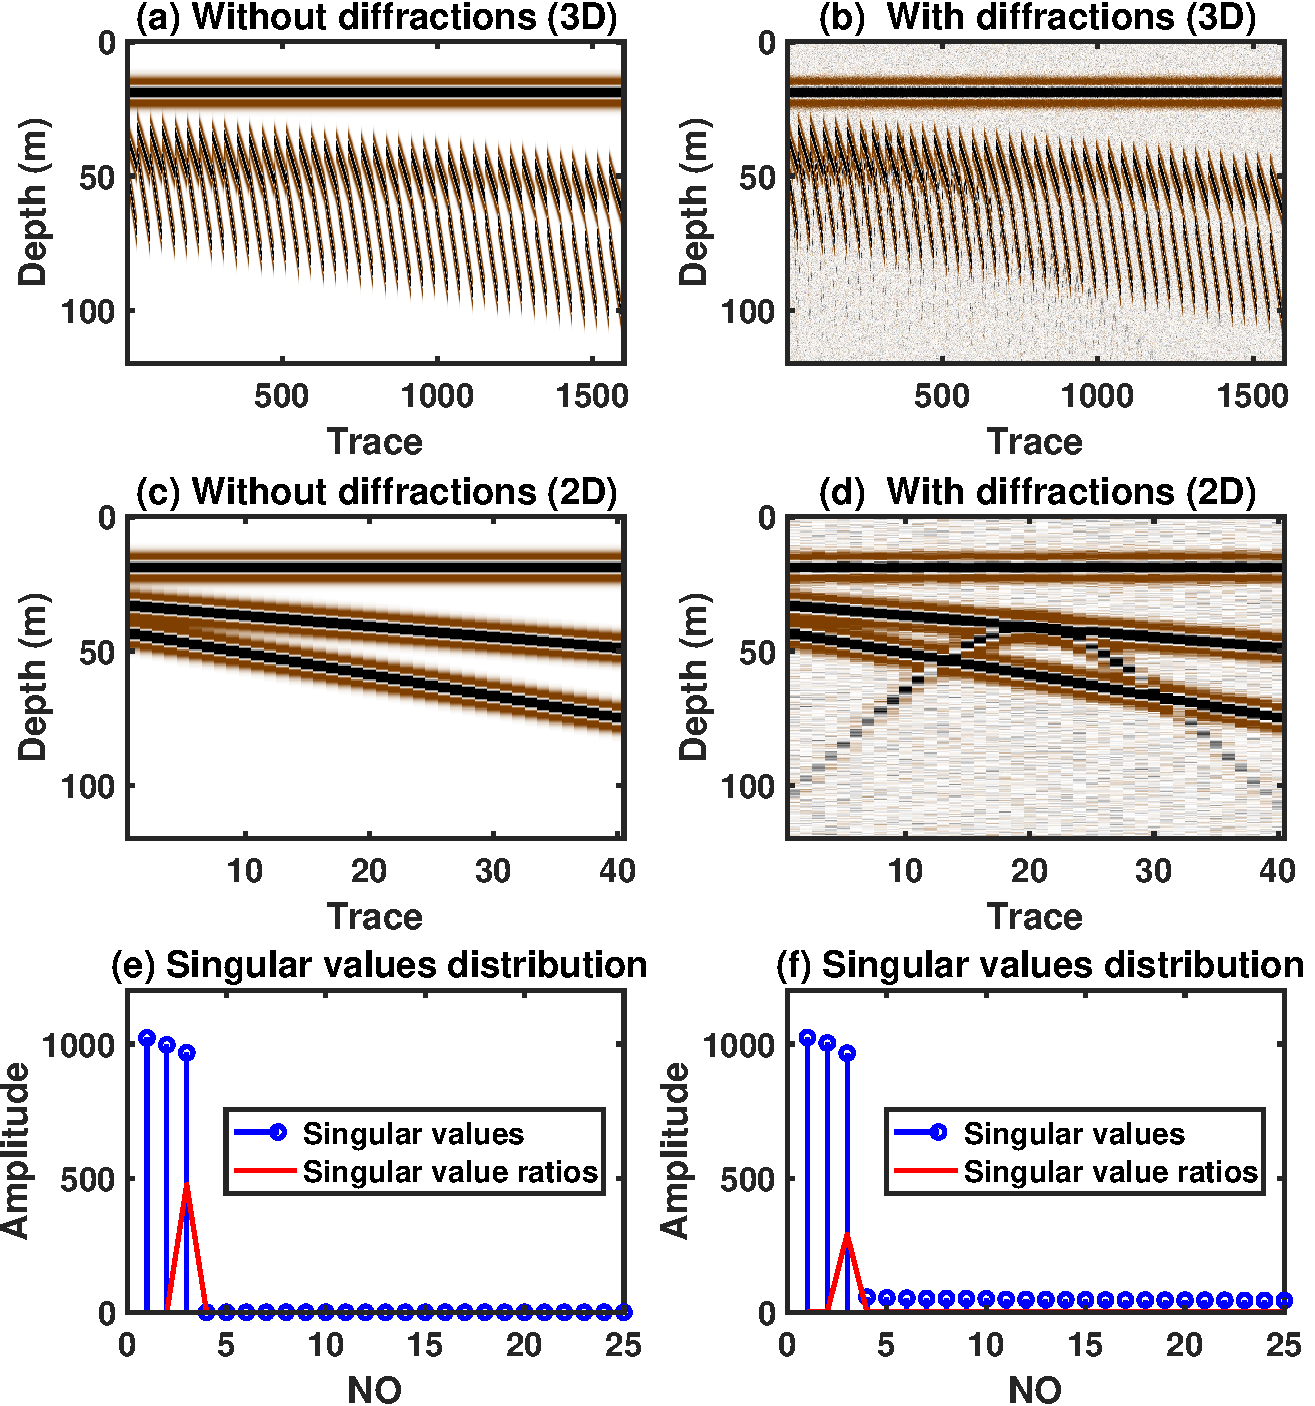
\includegraphics[width=\columnwidth]{Fig/demosigma}
%\caption{Singular value distribution. (a) 3D reflection data containing three plane waves. (b) 3D seismic data containing reflections, diffractions and random noise. (c) 2D section extracted from (a). (d) 2D section extracted from (b). (e) Singular values distribution of the Hankel matrix in the 20 Hz slice of the data shown in (a).  (f) Singular values distribution of the data shown in (b). }
%\label{fig:demosigma}
%\end{figure}
\inputdir{./}
\plot{demosigma}{width=\columnwidth}{Singular value distribution. (a) 3D reflection data containing three plane waves. (b) 3D seismic data containing reflections, diffractions and random noise. (c) 2D section extracted from (a). (d) 2D section extracted from (b). (e) Singular values distribution of the Hankel matrix in the 20 Hz slice of the data shown in (a).  (f) Singular values distribution of the data shown in (b). }
%\begin{figure}[htb!]
% \centering
% \subfigure[]{\includegraphics[width=0.31\columnwidth]{plot/Fig/refl}
%   \label{fig:refl}}
% \subfigure[]{\includegraphics[width=0.31\columnwidth]{plot/Fig/diffr}
%   \label{fig:diffr}}   
% \subfigure[]{\includegraphics[width=0.31\columnwidth]{plot/Fig/syn}
%   \label{fig:syn}}    
%\caption{Benchmark dataset with groundtruth reflections and diffractions. (a) Reflection data. (b) Diffraction data. (c) Synthetic data. }
%\label{fig:refl,diffr,syn}
%\end{figure}
%
%\begin{figure}[htb!]
% \centering
% \subfigure[]{\includegraphics[width=0.31\columnwidth]{plot/Fig/s-pwd-0}
%   \label{fig:s-pwd-0}}
% \subfigure[]{\includegraphics[width=0.31\columnwidth]{plot/Fig/s-grr-0}
%   \label{fig:s-grr-0}}   
% \subfigure[]{\includegraphics[width=0.31\columnwidth]{plot/Fig/s-lrra-0}
%   \label{fig:s-lrra-0}}    
%\caption{Separated reflections using (a) PWD method, (b) global rank-reduction method, and (c) proposed method.}
%\label{fig:s-pwd-0,s-grr-0,s-lrra-0}
%\end{figure}
%
%\begin{figure}[htb!]
% \centering
% \subfigure[]{\includegraphics[width=0.31\columnwidth]{plot/Fig/s-pwd-n-0}
%   \label{fig:s-pwd-n-0}}
% \subfigure[]{\includegraphics[width=0.31\columnwidth]{plot/Fig/s-grr-n-0}
%   \label{fig:s-grr-n-0}}   
% \subfigure[]{\includegraphics[width=0.31\columnwidth]{plot/Fig/s-lrra-n-0}
%   \label{fig:s-lrra-n-0}}    
%\caption{Separated diffractions using (a) PWD method (SNR=6.52 dB), (b) global rank-reduction method (SNR=1.42 dB), and (c) proposed method (SNR=9.14 dB).}
%\label{fig:s-pwd-n-0,s-grr-n-0,s-lrra-n-0}
%\end{figure}
%
%\begin{figure}[htb!]
%\centering
%\subfigure[]{\includegraphics[width=0.31\columnwidth]{plot/Fig/s-pwd-e-0}
%  \label{fig:s-pwd-e-0}}
%\subfigure[]{\includegraphics[width=0.31\columnwidth]{plot/Fig/s-grr-e-0}
%  \label{fig:s-grr-e-0}}   
%\subfigure[]{\includegraphics[width=0.31\columnwidth]{plot/Fig/s-lrra-e-0}
%  \label{fig:s-lrra-e-0}}    
%\caption{\new{Error of separated diffractions using (a) PWD method, (b) global rank-reduction method, and (c) proposed method.} \color{black}{}}
%\label{fig:s-pwd-e-0,s-grr-e-0,s-lrra-e-0}
%\end{figure}

\inputdir{syn3d}
\multiplot{3}{refll,diffrr,syn3d2}{width=0.45\columnwidth}{Benchmark dataset with groundtruth reflections and diffractions. (a) Reflection data. (b) Diffraction data. (c) Synthetic data. }
\multiplot{3}{s-pwd-0,s-grr-0,s-lrra-0}{width=0.45\columnwidth}{Separated reflections using (a) PWD method, (b) global rank-reduction method, and (c) proposed method.}
\multiplot{3}{s-pwd-n-0,s-grr-n-0,s-lrra-n-0}{width=0.45\columnwidth}{Separated reflections using (a) PWD method (SNR=6.52 dB), (b) global rank-reduction method (SNR=1.42 dB), and (c) proposed method (SNR=9.14 dB).}
\multiplot{3}{s-pwd-e-0,s-grr-e-0,s-lrra-e-0}{width=0.45\columnwidth}{Error of separated diffractions using (a) PWD method, (b) global rank-reduction method, and (c) proposed method.}


\section*{THEORY AND Methods}
Diffraction separation can be regarded as a problem of seismic data reconstruction, in which diffractions are treated as effective signals while reflections are treated as noise.  In the post-stack seismic data, reflections appear as locally linear events, while diffractions behave as hyperbolic events.  The rank-reduction method can utilize the kinematic differences between diffractions and reflections to separate different components. Besides, the energy of diffractions is much weaker than that of reflections, thereby corresponding to different singular values and singular vectors. The distributions of singular values for diffractions and reflections are assumed to be disparate in the singular-value spectrum. Therefore, the contribution of the last few singular values is the smallest, while the first few singular values contribute more to reconstructing the data. The rank-reduction method also considers the energy discrepancy, i.e., the dynamic differences, to separate weak diffractions and strong reflections \cite[]{2010Separation, 2016Diffraction}.    

\subsection{Local rank-reduction method}
Let a 3D seismic data be denoted by $S(x, y, t)$, $x=1,\cdots, N_x$, $y=1,\cdots, N_y$, and $t=1,\cdots, N_t$, where $N_x$, $N_y$ and $N_t$ represent the numbers of samples in spatial and time axes, respectively. The rank-reduction method \cite[]{2011Simultaneous,weilin2016dmssa} is implemented in the frequency domain, thus the first step is to obtain the corresponding frequency-domain data $S(x, y,f )$  by forward Fourier transform $\mathcal{F}$. For a given frequency $f_0$, we construct the block Hankel matrix $\mathbf{{H}}$ by mapping the frequency-domain data into several Hankel matrices $\mathbf{\widetilde{H}}_i(f_0)$ through the Hankelization operator $\mathcal{H}$. Then, we can obtain,
\begin{align} \label{eq:B} 
\mathbf{{H}}=
\begin{bmatrix}
\mathbf{\widetilde{H}}_1(f_0)&\mathbf{\widetilde{H}}_2(f_0)&\cdots&\mathbf{\widetilde{H}}_{n_x}(f_0)\\
\mathbf{\widetilde{H}}_2(f_0)&\mathbf{\widetilde{H}}_3(f_0)&\cdots&\mathbf{\widetilde{H}}_{n_x+1}(f_0)\\
\vdots&\vdots&\ddots&\vdots\\
\mathbf{\widetilde{H}}_{m_x}(f_0)&\mathbf{\widetilde{H}}_{m_x+1}(f_0)&\cdots&\mathbf{\widetilde{H}}_{m_x}(f_0)
\end{bmatrix}
,
\end{align}
where, 
\begin{align} \label{eq:Hif} 
&\mathbf{\widetilde{H}}_i(f_0)=\\
&\begin{bmatrix}
S(i,1,f_0)&S(i,2,f_0)&\cdots&S(i,n_y,f_0)\\
S(i,2,f_0)&S(i,3,f_0)&\cdots&S(i,n_y+1,f_0)\\
\vdots&\vdots&\ddots&\vdots\\
S(i,m_y,f_0)&S(i,m_y+1,f_0)&\cdots&S(i,N_y,f_0)
\end{bmatrix}
,
\end{align}
$m_x=\text{INT}(N_x/2)+1$ and $n_x=N_x-m_x+1$ are the key parameters to make the block Hankel matrix close to a square matrix. Similarly, $m_y=\text{INT}(N_y/2)+1$ and $n_y=N_y-m_y+1$.  $\text{INT}(\cdot)$ represents the integer part of an argument. 

\cite[]{Zheng2014A} point out that the component with strong energy corresponds to a large singular value, i.e., the strong signals correspond to large singular values. On the contrary, the smaller singular values represent the energy of diffractions and noise. 
It is straightforward to infer that the largest singular values of block Hankel matrix represent the reflections.  If we can obtain the reflection wave $\mathbf{R}$ by extracting the corresponding singular values and vectors, then the diffraction wave $\mathbf{D}$ can be obtained by subtracting $\mathbf{R}$ from the data $\mathbf{S}$,
\begin{equation}\label{eq:dsr}
\mathbf{D}=\mathbf{S}-\mathbf{R}.
\end{equation}

Thus, the problem of diffraction separation is transformed into estimating the reflection, which can be addressed by applying the singular-value decomposition (SVD) algorithm to the block Hankel matrix \cite[]{Chen2016An}. In particular, truncated singular-value decomposition (TSVD) is usually used to suppress the noise. The TSVD of block Hankel matrix is expressed as
\begin{equation} \label{eq:svd}
\mathbf{\hat{H}}=\mathbf{U}\mathbf{\Sigma}\mathbf{V}^T,
\end{equation}
where $\mathbf{\hat{H}}$ denotes the denoised block Hankel matrix, i.e., the noise can be suppressed by ignoring some smaller singular values \cite[]{2020Diffraction}.  $\mathbf{\Sigma}=[{\sigma}_1,{\sigma}_2,\cdots,{\sigma}_N]$ is the diagonal singular matrix, $\mathbf{U}=[\mathbf{u}_1,\mathbf{u}_2,\cdots,\mathbf{u}_N]$ and $\mathbf{V}=[\mathbf{v}_1,\mathbf{v}_2,\cdots,\mathbf{v}_N]$ are left and right singular matrices, respectively. They are made up of singular vectors $\mathbf{u}_j$ and $\mathbf{v}_j$. $\sigma_j$ denotes the $j$th singular value, and $N$ denotes the number of singular values.

Then, we can reconstruct the block Hankel matrix of reflections $\mathbf{H}_R$ by selecting an appropriate rank $R$, which will be introduced in detail in the following section. After that, the inverse Hankelization operator $\mathcal{H}^{-1}$ and inverse Fourier transform $\mathcal{F}^{-1}$ are implemented to obtain reflections in time-domain. 
The processes can be expressed as,
%\begin{equation}
%\begin{array}{c}
\begin{align}\label{eq:rtime}
\begin{split}
\mathbf{R}&= \mathcal{F}^{-1} \mathcal{H}^{-1}\mathbf{H}_R\\ 
&= \mathcal{F}^{-1} \mathcal{H}^{-1}\mathcal{T}\mathbf{\hat{H}}\\ 
&= \mathcal{F}^{-1} \mathcal{H}^{-1}\mathcal{T}\mathcal{H}\mathbf{S}_F\\ 
&=\mathcal{F}^{-1} \mathcal{H}^{-1} \mathcal{T}\mathcal{H}\mathcal{F}\mathbf{S}, 
\end{split}
\end{align}
%\end{array}
%,
%\end{equation}
where $\mathcal{T}$ represents the principal component extraction operator, $\mathbf{S}$ and $\mathbf{S}_F$ represent the data in time- and frequency-domain, respectively. The reconstructed block Hankel matrix of reflections $\mathbf{H}_R$ is given by,
\begin{equation}\label{eq:HR}
\mathbf{H}_R=\mathcal{T}\mathbf{\hat{H}}=\sum^R \limits_{r=1} {\sigma}_r\mathbf{u}_r\mathbf{v}_r^\text{T}.
\end{equation}

It can seen from equation \ref{eq:HR} that it is important to determine whether the  singular value corresponds to diffraction or reflection, i.e., selecting appropriate rank values for rank reduction, especially for the singular values near the intersection of reflections and diffractions. Since the assumption of plane waves is only satisfied locally, it is advisable to perform the rank reduction in local windows to boost the performance for the complexity of 3D seismic data, i.e., the LRR method. Let $\mathcal{W}$ and $\mathcal{W}^{-1}$ represent the windowing and reconstruction operators, then the reconstructed reflections by using LRR can be written in operator notation as,
\begin{equation} \label{eq:wr}
\mathbf{R}=\mathcal{W}^{-1}\mathcal{F}^{-1} \mathcal{H}^{-1} \mathcal{T}\mathcal{H}\mathcal{F}\mathcal{W}\mathbf{S}.
\end{equation}


%\begin{figure}[htb!]
% \centering
% \subfigure[]{\includegraphics[width=0.6\columnwidth]{plot/Fig/ovp}
%   \label{fig:ovp}}
% \subfigure[]{\includegraphics[width=0.6\columnwidth]{plot/Fig/o}
%   \label{fig:o}}     
%\caption{(a) Velocity model of the first synthetic example. (b) Zero-offset data simulated from the velocity model.}
%\label{fig:ovp,o}
%\end{figure}
%
%\begin{figure}[htb!]
% \centering
% \subfigure[]{\includegraphics[width=0.31\columnwidth]{plot/Fig/o-pwd}
%   \label{fig:o-pwd}}
% \subfigure[]{\includegraphics[width=0.31\columnwidth]{plot/Fig/o-lrr}
%   \label{fig:o-lrr}}   
% \subfigure[]{\includegraphics[width=0.31\columnwidth]{plot/Fig/o-lrra}
%   \label{fig:o-lrra}} \\
% \subfigure[]{\includegraphics[width=0.31\columnwidth]{plot/Fig/o-pwd-n-0}
%   \label{fig:o-pwd-n-0}}
% \subfigure[]{\includegraphics[width=0.31\columnwidth]{plot/Fig/o-lrr-n-0}
%   \label{fig:o-lrr-n-0}}   
% \subfigure[]{\includegraphics[width=0.31\columnwidth]{plot/Fig/o-lrra-n-0}
%   \label{fig:o-lrra-n-0}}    
%\caption{First row: separated reflection data using (a) the PWD method, (b) the LRR method, and (c) the LRRA method. Second row: separated diffractions using (d) the PWD method, (e) the LRR method, and (f) the LRRA method.}
%\label{fig:o-pwd,o-lrr,o-lrra,o-pwd-n-0,o-lrr-n-0,o-lrra-n-0}
%\end{figure}
%
%\begin{figure}[htb!]
% \centering
% \subfigure[]{\includegraphics[width=0.31\columnwidth]{plot/Fig/o-pwd-imag-0}
%   \label{fig:o-pwd-imag-0}}
% \subfigure[]{\includegraphics[width=0.31\columnwidth]{plot/Fig/o-lrr-imag-0}
%   \label{fig:o-lrr-imag-0}}   
% \subfigure[]{\includegraphics[width=0.31\columnwidth]{plot/Fig/o-lrra-imag-0}
%   \label{fig:o-lrra-imag-0}}    
%\caption{Migrated diffraction image using (a) the PWD method, (b) the LRR method, and (c) the LRRA method. The arrows indicate less reflection energy and higher resolution using the LRRA method.}
%\label{fig:o-pwd-imag-0,o-lrr-imag-0,o-lrra-imag-0}
%\end{figure}


\subsection{Rank estimation in local windows}
Selecting an appropriate rank for each window is crucial in reflection reconstruction and diffraction separation. 
It is the key to judge whether a singular value corresponds to the reflection energy or the diffraction energy.
As the 3D seismic data are divided into various sub-volumes, it is necessary to independently estimate the rank for each local volumes. 
The common practice is specifying a threshold, and comparing the singular values with the threshold. 
If the singular values are larger than the threshold, they are regarded to correspond to reflections, thereby being preserved.
On the contrary, the residual singular values correspond to diffractions.
A small rank means that the disregarded energy is relatively large, then the reflection may exists in the separated diffractions.
A large value of threshold will damage the diffraction energy because a part of the diffraction energy is mixed in the  reconstructed reflections.
Consequently,  the determination of rank values is challenging, and conventional strategies, such as  the difference curvature method \cite[]{Vicente2011Simultaneous}, may be artificial. 
Besides, it is difficult and time-consuming to manually specify a rank value in each local window.
Based on the complexity of the 3D seismic volumes, we propose an adaptive and automatic method to determine the rank values in different windows.
Let us consider the singular value ratio in a window, which is given by
\begin{equation} \label{eq:svr}
V_i=\dfrac{\sigma_i}{\sigma_{i+1}},i=1,2,\cdots,L-1,
\end{equation}
where $V_i$ denotes the singular value ratio sequence from large to small and $L$ is the length of the singular spectrum. Then, we can estimate the rank $\hat{R}$ of a local window by selecting the maximum of  the singular value ratio sequence, 
\begin{equation} \label{eq:svr}
\hat{R}=\text{arg} \max\limits_i\quad V_i.
\end{equation}
Taking $\hat{R}$ into equation \ref{eq:HR}, we can separate diffractions and reflections according to equations \ref{eq:wr} and \ref{eq:dsr}. 

We summarize the procedures of the proposed new method for diffraction separation as the following steps,
\begin{enumerate}
\item dividing the 3D seismic data into several volumes by sliding the local window,
\item transforming the time-domain data into frequency domain by using Fourier transform,
\item mapping the frequency-domain data into a block Hankel matrix,
\item applying the TSVD algorithm to the block Hankel matrix,
\item estimating the rank by using the proposed automatic determination approach,
\item reconstructing the block Hankel matrix of reflections by inverse Hankelization operator,
\item applying the inverse Fourier transform and aggregating all reflection volumes in different windows,
\item subtracting the reflections from the 3D seismic data and obtaining the diffractions. 
\end{enumerate}
We called the proposed automated local method the LRR method with adaptively selected ranks (LRRA). 

To demonstrate the feasibility of the singular value ratios as an effective rank selection strategy, we conduct a simple test, where we create a synthetic reflection dataset with three plane waves and add a diffraction wave to it to see how the singular values vary with and without the diffraction wave. We also add some weak random noise to mimic the real situation. The 3D datasets without and with diffractions are plotted in Figures \ref{fig:demosigma}(a) and \ref{fig:demosigma}(b), respectively. Here, we plot the 3D data as a 2D matrix to see the details inside the data. To clearly visualize the diffraction wave, we also plot the 2D sections from the 3D datasets in Figures  \ref{fig:demosigma}(c) (without the diffraction) and \ref{fig:demosigma}(d)  (with the diffraction), where one can see the bow-tie-like diffraction wave clearly. We plot the first 25 singular values of the block Hankel matrix of 20 Hz in Figures \ref{fig:demosigma}(e) (without the diffraction) and \ref{fig:demosigma}(f)  (with the diffraction). The blue dots correspond to the singular values and the red curves correspond to the singular value ratios. From Figure \ref{fig:demosigma}(e), it is clear that when there are no diffractions, there are only three non-zero singular values, and the maximum of singular value ratios correctly picks the correct rank of this data. From Figure \ref{fig:demosigma}(f), it is clear that when there is a diffraction wave, there are still three distinctively large singular values, with other singular values close to zeros. It is obvious that the energy of the diffraction wave and the random noise is mainly spreading in the singular values after the three largest values. The maximum of the singular value ratios correctly picks the correct rank again despite the existence of the diffraction wave and random noise. This test shows that the singular value ratio is an effective way to automatically distinguish between reflections and diffractions in the singular spectrum. 


%\begin{figure}[htb!]
% \centering
% \subfigure[]{\includegraphics[width=0.6\columnwidth]{plot/Fig/kvp}
%   \label{fig:kvp}}
% \subfigure[]{\includegraphics[width=0.6\columnwidth]{plot/Fig/k}
%   \label{fig:k}}     
%\caption{(a) Velocity model of the second synthetic example. (b) Zero-offset data simulated from the velocity model.}
%\label{fig:kvp,k}
%\end{figure}
%
%\begin{figure}[htb!]
% \centering
% \subfigure[]{\includegraphics[width=0.31\columnwidth]{plot/Fig/k-pwd}
%   \label{fig:k-pwd}}
% \subfigure[]{\includegraphics[width=0.31\columnwidth]{plot/Fig/k-lrr}
%   \label{fig:k-lrr}}   
% \subfigure[]{\includegraphics[width=0.31\columnwidth]{plot/Fig/k-lrra}
%   \label{fig:k-lrra}} \\
% \subfigure[]{\includegraphics[width=0.31\columnwidth]{plot/Fig/k-pwd-n-0}
%   \label{fig:k-pwd-n-0}}
% \subfigure[]{\includegraphics[width=0.31\columnwidth]{plot/Fig/k-lrr-n-0}
%   \label{fig:k-lrr-n-0}}   
% \subfigure[]{\includegraphics[width=0.31\columnwidth]{plot/Fig/k-lrra-n-0}
%   \label{fig:k-lrra-n-0}}    
%\caption{First row: separated reflection data using (a) the PWD method, (b) the LRR method, and (c) the LRRA method. Second row: separated diffractions using (d) the PWD method, (e) the LRR method, and (f) the LRRA method.}
%\label{fig:k-pwd,k-lrr,k-lrra,k-pwd-n-0,k-lrr-n-0,k-lrra-n-0}
%\end{figure}
%
%\begin{figure}[htb!]
% \centering
% \subfigure[]{\includegraphics[width=0.31\columnwidth]{plot/Fig/k-pwd-imag-0}
%   \label{fig:k-pwd-imag-0}}
% \subfigure[]{\includegraphics[width=0.31\columnwidth]{plot/Fig/k-lrr-imag-0}
%   \label{fig:k-lrr-imag-0}}   
% \subfigure[]{\includegraphics[width=0.31\columnwidth]{plot/Fig/k-lrra-imag-0}
%   \label{fig:k-lrra-imag-0}}    
%\caption{Migrated diffraction image using (a) the PWD method, (b) the LRR method, and (c) the LRRA method. The arrows indicate less reflection energy and higher resolution using the LRRA method.}
%\label{fig:k-pwd-imag-0,k-lrr-imag-0,k-lrra-imag-0}
%\end{figure}

%uncomment
\inputdir{o}
\multiplot{2}{ovp,o}{width=0.6\columnwidth}{(a) Velocity model of the first synthetic example. (b) Zero-offset data simulated from the velocity model.}

\multiplot{6}{o-pwd,o-lrr,o-lrra,o-pwd-n-0,o-lrr-n-0,o-lrra-n-0}{width=0.3\columnwidth}{First row: separated reflection data using (a) the PWD method, (b) the LRR method, and (c) the LRRA method. Second row: separated diffractions using (d) the PWD method, (e) the LRR method, and (f) the LRRA method.}

\multiplot{3}{o-pwd-imag-0,o-lrr-imag-0,o-lrra-imag-0}{width=0.45\columnwidth}{Migrated diffraction image using (a) the PWD method, (b) the LRR method, and (c) the LRRA method. The arrows indicate less reflection energy and higher resolution using the LRRA method.}

\inputdir{k}
\multiplot{2}{kvp,k}{width=0.6\columnwidth}{(a) Velocity model of the second synthetic example. (b) Zero-offset data simulated from the velocity model.}

\multiplot{6}{k-pwd,k-lrr,k-lrra,k-pwd-n-0,k-lrr-n-0,k-lrra-n-0}{width=0.3\columnwidth}{First row: separated reflection data using (a) the PWD method, (b) the LRR method, and (c) the LRRA method. Second row: separated diffractions using (d) the PWD method, (e) the LRR method, and (f) the LRRA method.}

\multiplot{3}{k-pwd-imag-0,k-lrr-imag-0,k-lrra-imag-0}{width=0.45\columnwidth}{Migrated diffraction image using (a) the PWD method, (b) the LRR method, and (c) the LRRA method. }




\section{Examples}
In this part, we will first benchmark the proposed method with two state-of-the-art methods, i.e., the PWD method \cite[]{2007Post} and the global rank-reduction (GRR) method \cite[]{2020Diffraction}, based on a relatively simple but representative 3D dataset. Then, we will test the effects of the diffraction separation methods on diffraction imaging of two 3D synthetic models. Finally, we will test the proposed method on a 3D field data example. 

\subsection{Benchmark comparison}
We create a 3D synthetic dataset for comparing the diffraction separation performance of different methods. In this comparison, since we have the ground truth diffractions and reflections, we can quantitatively compare different methods based on the signal-to-noise ratio (SNR) metric shown below.
\begin{equation}
\label{eq:snr}
\text{SNR}=10\log_{10}\frac{\Arrowvert \mathbf{d} \Arrowvert_2^2}{\Arrowvert \mathbf{d} -\mathbf{d}_s\Arrowvert_2^2},
\end{equation}
where $\mathbf{d}$ denotes the vectorized ground-truth diffraction and $\mathbf{d}_s$ corresponds to the separated diffraction.  

The synthetic reflections and diffractions are plotted in Figures \ref{fig:refl} and \ref{fig:diffr}, respectively. Figure \ref{fig:syn} shows the synthetic data containing both reflections and diffractions, i.e., the summation between Figures \ref{fig:refl} and \ref{fig:diffr}. The data size of this example is $200\times 100\times 100$. We simulate the diffraction waves by putting 16 evenly distributed diffraction points and use the kirchhoff modeling method to simulate both reflection and diffraction waves. We compare the separated reflections and diffractions using three methods, i.e., PWD, GRR, and the proposed methods, in Figures \ref{fig:s-pwd-0,s-grr-0,s-lrra-0} and \ref{fig:s-pwd-n-0,s-grr-n-0,s-lrra-n-0}. 
In the separated reflections shown in Figure \ref{fig:s-pwd-0,s-grr-0,s-lrra-0}, it is clear that all three methods separate most diffractions, but the GRR method causes significant residual diffractions in the reflections, as indicated by the arrows in Figure \ref{fig:s-grr-0}. 
It is easier for comparing different methods in the separated diffraction cubes in Figure \ref{fig:s-pwd-n-0,s-grr-n-0,s-lrra-n-0}, where the damages to reflection waves and the energy difference of the separated diffractions can be seen clearly. In Figure \ref{fig:s-pwd-n-0}, there are obvious reflections in the diffractions, indicating the serious coupling between reflections and diffractions after separation. Figure \ref{fig:s-grr-n-0} shows obviously weaker diffractions, indicating the strong residual diffractions in the reflections. The proposed method, however, obtains a good separation between reflections and diffractions. In this benchmark test, the parameters of different methods have been tuned to output the highest SNRs. The GRR method uses a global rank of 60, and the proposed method uses a window size of 40 samples in both spatial directions. The SNRs of the results from PWD, GRR, and the proposed method are 6.52 dB, 3.14 dB, and 9.14 dB, respectively, as compared to -28.23 dB of the input data containing the whole reflection data. \new{The error cubes of estimated diffractions are plotted in Figure \ref{fig:s-pwd-e-0,s-grr-e-0,s-lrra-e-0}, where it is clear that the proposed method obtains the smallest error.}








\subsection{Synthetic diffraction imaging test}
The first diffraction imaging test is based on the Ordovician model \cite[]{decker2015carbonate,janson2010ultra,decker2015carbonate}. This model 
is built based on the Ordovician limestone strata located in Tarim Basin, China, to test the diffraction imaging methods in characterizing paleokarst features in very deeply buried strata. The velocity model follows the Ordovician unconformity surface (between the basal Ordovician layer and the overlying siliciclastic Silurian layer) that is mapped from active-source reflection seismic data.  The paleo-caves are collapsed due to the deposition of sediments, which are modeled by randomly distributing the low acoustic impedance anomalies in the 3D model. The paleo-caves have a general size of 18 m in vertical slices and 300 $\times$ 300 m in horizontal slices. We show the velocity model ($416\times200\times 200$) in Figure \ref{fig:ovp}. Figure \ref{fig:o} plots the simulated zero-offset seismic data ($1351\times200\times 128$). The bow-tie-like diffractions are very obvious in the data. Figure \ref{fig:o-pwd,o-lrr,o-lrra,o-pwd-n-0,o-lrr-n-0,o-lrra-n-0} shows the comparison of separated reflections and diffractions. Figures \ref{fig:o-pwd}-\ref{fig:o-lrra} plot the separated reflections using the PWD, LRR, and the proposed methods, respectively. In both LRR and LRRA methods, we use a window size of 50 samples in both inline and crossline directions. Figures \ref{fig:o-pwd-n-0}-\ref{fig:o-lrra-n-0} plot their corresponding diffractions. Comparing the separated diffractions, it is clear that the PWD method tends to remove reflections when separating the diffractions, as indicated by the arrows. The diffractions separated by the LRR method without a proper selection of the rank are obviously weaker.  The proposed LRRA method (see Figure \ref{fig:o-lrra}), however, obtains good results. The migrated images using the separated diffractions are compared in Figure \ref{fig:o-pwd-imag-0,o-lrr-imag-0,o-lrra-imag-0}. It is clear that the image using the PWD method contains some energy corresponding to the reflections (see the arrows). The LRR method (Figure \ref{fig:o-lrr-imag-0}) obtains a more vague image than the other two methods. The proposed LRRA method (Figure \ref{fig:o-lrra-imag-0}), however, obtains a clear image of the paleo-caves. 






The second diffraction imaging test is based on the Khuff model \cite[]{decker2015carbonate,janson2013outcrop}, which corresponds to the Permian-Triassic Khuff reservoir that crops out in central Saudi Arabia near Buraydah. This model was originally built to study the influence of small-scale heterogeneities in carbonate reservoirs on the subsurface flow models \cite[]{janson2013outcrop}. The velocity ($380\times200\times 128$) is plotted in Figure \ref{fig:kvp}. Figure \ref{fig:k} plots the numerically modelled zero-offset data ($400\times200\times 128$), where the bow-tie-like diffractions are evident. Figures \ref{fig:k-pwd}-\ref{fig:k-lrra} compare the separated reflections using the PWD, LRR, and LRRA methods.  All three methods obtain smooth reflections with most diffractions separated. Figures \ref{fig:k-pwd-n-0}-\ref{fig:k-lrra-n-0} compare the separated diffractions. It is clear that Figure \ref{fig:k-pwd-n-0} contains significant spatially coherent reflection waves, indicating a strong coupling between diffractions and reflections using the PWD method. The clear reflection energy is highlighted by the arrows in Figure \ref{fig:k-pwd-n-0}. Figure \ref{fig:k-lrr-n-0} has much weaker diffraction energy, indicating the less competent ability of the LRR method in separating the diffractions without a properly chosen rank parameter. The LRRA method, as plotted in Figure \ref{fig:k-lrra-n-0}, obtains better performance compared with the other two methods. Figure \ref{fig:k-pwd-imag-0,k-lrr-imag-0,k-lrra-imag-0} compares  the diffraction imaging results using three different methods. In both LRR and LRRA methods, we use a window size of 50 samples in the inline direction and a window size of 64 samples in the crossline direction. It is obvious that the PWD method causes obvious reflection structures (see the arrows in Figure \ref{fig:k-pwd-imag-0}), while the LRR method fails in separating all the diffractions, thereby causing less clear depictions of the small-scale heterogeneities. The LRRA method obtains a clearly better result.  






\subsection{Field data example}
Next, we apply the proposed method to a 3D field dataset. \new{It is a land seismic dataset from the Cooper Basin in Western Australia, which was used to characterize the tight-gas sand reservoir. Some previous studies regarding this dataset have been published in \cite[]{merzlikin2017analytical} and \cite[]{tyiasning2016comparison}.} \new{Detailed geological description of the area as well as the comparison of diffraction imaging results to discontinuity-type attributes is given by \cite[]{tyiasning2016comparison}. \new{In particular, this dataset has fully azimuthal distribution of offsets and a far offset of 4000 m. The horizon maps shown below come from an interface between a pervasive sheet coal and fluvial Permian Patchawarra Sand at a depth of approximately 2500 m \cite[]{tyiasning2016comparison}.} The Patchawarra Sand is a tight-gas sand at this field.} The 3D post-stack dataset is plotted in Figure \ref{fig:b}. Figures \ref{fig:b-pwd}-\ref{fig:b-lrra} plot the separated reflection data using the PWD, LRR, and LRRA methods, respectively. In both LRR and LRRA methods, we use a window size of 50 samples in both inline and crossline directions.  Correspondingly, we show the separated diffractions in Figure \ref{fig:b-pwd-n-0,b-lrr-n-0,b-lrra-n-0}, where it is clear that the LRR method fails in separating sufficient amount of diffractions.  Although the PWD method succeeds in separating the diffractions, it also tends to remove the reflections, which are more spatially coherent than the diffractions, as indicated by the arrows. The labeled arrow indicates a noticeable area of the crossline-coherent reflections. The crossline-coherent reflection refers to the reflection energy that is coherent only in the crossline direction and is incoherent in the inline direction. To better visualize the difference of the separated diffractions in a horizontal slice, we extract a time slice (t=1.7 s) from the diffraction cubes and show the comparison in Figure \ref{fig:b-pwd-n-t-0,b-lrr-n-t-0,b-lrra-n-t-0}, where it is clearer to see the reflection energy using the PWD method. We migrate the separated diffractions using an analytical path-summation imaging method \cite[]{merzlikin2017analytical}, and show an extracted time slice in Figure \ref{fig:b-pwd-rimag-0,b-pwd-imag-0,b-lrr-imag-0,b-lrra-imag-0}. Apart from the diffraction images, we also show a conventional reflection image in Figure \ref{fig:b-pwd-rimag-0} for evaluating the advantage of the diffraction imaging in delineating small-scale heterogeneities. It is clear that the diffraction image using the PWD method is more consistent with the reflection image, e.g., the area pointed out by the labeled arrow. The highlighted area by the arrows shows a crossline-oriented paleo-channel, which can be captured by both reflection and diffraction images. However, this consistency does not demonstrate the advantage of the diffraction imaging, which, instead, indicates the deficiency of the PWD method in excluding the reflection waves that are coherent in one direction. The image using the LRRA method, however, does not show the clear paleo-channel that is more characterized by the reflection waves. From the general comparison in Figure \ref{fig:b-pwd-rimag-0,b-pwd-imag-0,b-lrr-imag-0,b-lrra-imag-0}, the image using the LRRA method has an obviously higher resolution in delineating the small-scale heterogeneities (viewed from all directions), such as the paleo-karsts. 

\section{Discussion}
%PWD
%parameter
%GRR
The PWD-based diffraction separation framework has been widely studied and used. While it has a superb capability in separating diffractions out from the post-stack seismic data, very little researches have been done to explore the shortcomings of this method. We have done many numerical as well as field data tests and found that the PWD-based method could suffer from the coupling effect between reflection and diffraction wave components. It is known that the PWD method is based on the local slope calculation and the spatial coherency difference between the reflections and diffractions. On the one hand, the slope estimation based on the PWD method suffers from the noise sensitivity, as reported in many previous studies \cite[]{shaohuan2017,wanghang2020tgrs2,chenwei2021geo,chenwei2021tgrs2}. The inaccurate slope estimation will affect the separation performance between diffractions and reflections, causing the coupling effect. On the other hand, the spatial coherency between diffractions and reflections is not always disparate, which will result in the coupling of them on the local slope estimation. In other words, when the diffractions and reflections are similar in terms of spatial coherency, the PWD method will also estimate the slope of the diffractions, making the separation algorithm treat both diffractions and reflections as signals and thereby causing either separated diffractions and reflections coupling together or an insufficient amount of separated diffraction energy. As can be seen in the aforementioned examples, the PWD method tends to cause a significant amount of reflection energy in the diffraction volumes, which further lowers the resolution of the diffraction image.

The rank-reduction method is a completely data-driven method that does not require an intermediate step like the PWD method. The difference between the reflections and diffractions is reflected in the amplitude distribution of singular values. Traditional rank-reduction methods rely on a manual selection of the rank parameter, which may involve several try-and-error steps. The general assumption is that the rank is equivalent to the number of distinct dipping components. It is valid for simple synthetic data with several plane waves. However, it is not applicable in complicated datasets where the seismic events are highly non-stationary. Thus, the assumption of the rank-reduction method is not valid for processing a large 3D realistic seismic dataset without applying the windowing strategy. Previous 2D diffraction imaging method based on the GRR method has shown some promising results \cite[]{2020Diffraction}, but causes significant artifacts due to the complication in the singular value distribution. The local rank-reduction method can help obtain better results because of the much-simplified data structure that follows the separation assumption. However, another problem arises due to the windowing strategy, i.e., the rank incoherency issue \cite[]{shaohuan2017gji,yangkang2017ieee}. The adaptive rank selection method proposed in this paper well solves the rank incoherency problem by adapting the local structure with the automatically chosen rank parameter. The proposed method is free of manual rank selection and thus is convenient to use. The only parameter required to adjust in the proposed framework is the window size. The window size here only refers to the spatial window size. Since the coherency to distinguish between diffractions and reflections is mainly related to the spatial dimension, we do not apply temporal window in the proposed framework. \new{In order to investigate how the spatial window can affect the diffraction separation performance, we conduct several tests based on the first benchmark example shown in Figure \ref{fig:refl,diffr,syn}.  We use different spatial window sizes to separate the diffractions and use the SNR to quantitatively evaluate the performance, and plot the SNR diagrams in Figure \ref{fig:curve}. Here, because our synthetic data is symmetric in the two spatial directions, we can only vary the window size in one spatial direction, and use the same value for the other direction.
In Figure \ref{fig:curve}, the horizontal axis corresponds to the window size, and the vertical axis corresponds to the SNR. It is clear that the SNR reaches the highest when the window size is 40 samples. It is clear that the 40 samples coincide with the spatial width of the bow-tie-like diffraction wave. Thus, we conclude from this test that the optimal window size should be chosen roughly as the spatial width of the observable diffraction wave component. }

\new{Existence of noise could affect the performance of the proposed method. If the noise is random, it will be combined with the diffraction energy as the output of the local rank-reduction method. It is possible to further separate the random noise from the diffraction energy by leveraging their differences in the singular spectrum \cite[]{weilin2017dlsp,oboue2021geo1,oboue2021geo2}. If the noise is random but linear, it will likely be considered as the diffraction energy, and could be interfering the separated diffraction energy when input to the imaging framework. However, it indeed depends on the spatial coherency difference between the linear noise and the diffraction energy. If the linear noise is steeply dipping and is more spatially incoherent than diffraction energy \cite[]{weilin2017mmf}, then the proposed method could still be effective in distinguishing the two components. }

The computational cost of the LRR method is much lower than the GRR method. The state-of-the-art rank-reduction method with a full singular value decomposition (SVD) has a computational cost of $O(N_1(N_2N_3)^3)$, and with a truncated SVD operation has a cost of $O(N_1K(N_2N_3)^2)$, where $N_i$ denotes the size of the $i$th dimension. $K$ denotes the rank parameter.
Thus, using a local rank-reduction method can also help significantly reduce the computational overburden. For the 3D examples presented in this paper, only the first synthetic example ($200\times 100\times 100$) can afford the global method, thus we present its result. For this test, the local method with a spatial window size of 40 samples takes 263.3 s, while the global method takes 3266.3 s. It is a speedup of 12.4 times. The computation is done on a Mac Pro laptop PC with 2.5 GHz Intel Core i7. For the other three datasets, the global method is prohibitively expensive, thus we do not show the results. Note that to further increase the computational efficiency, a randomized SVD can also be used to obtain a large speedup but at the expense of degrading the performance \cite[]{li2014large}. The automatic rank selection strategy almost adds no extra computational cost to the rank-reduction method, so the overall computational efficiency of the proposed method is acceptable. 

%\begin{figure}[htb!]
% \centering
% \subfigure[]{\includegraphics[width=0.48\columnwidth]{plot/Fig/b}
%   \label{fig:b}}
% \subfigure[]{\includegraphics[width=0.48\columnwidth]{plot/Fig/b-pwd}
%   \label{fig:b-pwd}}    \\
% \subfigure[]{\includegraphics[width=0.48\columnwidth]{plot/Fig/b-lrr}
%   \label{fig:b-lrr}}    
% \subfigure[]{\includegraphics[width=0.48\columnwidth]{plot/Fig/b-lrra}
%   \label{fig:b-lrra}} 
%\caption{Field data example. (a) A 3D field dataset. Separated reflection data using (b) the PWD method, (c) the LRR method, and (d) the LRRA method. }
%\label{fig:b,b-pwd,b-lrr,b-lrra}
%\end{figure}
%\begin{figure}[htb!]
% \centering
% \subfigure[]{\includegraphics[width=0.48\columnwidth]{plot/Fig/b-pwd-n-0}
%   \label{fig:b-pwd-n-0}}
% \subfigure[]{\includegraphics[width=0.48\columnwidth]{plot/Fig/b-lrr-n-0}
%   \label{fig:b-lrr-n-0}}   
% \subfigure[]{\includegraphics[width=0.48\columnwidth]{plot/Fig/b-lrra-n-0}
%   \label{fig:b-lrra-n-0}}    
%\caption{Separated diffraction data using (a) the PWD method, (b) the LRR method, and (c) the LRRA method.}
%\label{fig:b-pwd-n-0,b-lrr-n-0,b-lrra-n-0}
%\end{figure}
%\begin{figure}[htb!]
% \centering
% \subfigure[]{\includegraphics[width=0.48\columnwidth]{plot/Fig/b-pwd-n-t-0}
%   \label{fig:b-pwd-n-t-0}}
% \subfigure[]{\includegraphics[width=0.48\columnwidth]{plot/Fig/b-lrr-n-t-0}
%   \label{fig:b-lrr-n-t-0}}   
% \subfigure[]{\includegraphics[width=0.48\columnwidth]{plot/Fig/b-lrra-n-t-0}
%   \label{fig:b-lrra-n-t-0}}    
%\caption{A comparison of time slices extracted from the separated diffraction data using (a) the PWD method, (b) the LRR method, and (c) the LRRA method. }
%\label{fig:b-pwd-n-t-0,b-lrr-n-t-0,b-lrra-n-t-0}
%\end{figure}
%\begin{figure}[htb!]
%\centering
%\subfigure[]{\includegraphics[width=0.48\columnwidth]{plot/Fig/b-pwd-rimag-0}
%  \label{fig:b-pwd-rimag-0}}
%\subfigure[]{\includegraphics[width=0.48\columnwidth]{plot/Fig/b-pwd-imag-0}
%  \label{fig:b-pwd-imag-0}} \\
%\subfigure[]{\includegraphics[width=0.48\columnwidth]{plot/Fig/b-lrr-imag-0}
%  \label{fig:b-lrr-imag-0}}   
%\subfigure[]{\includegraphics[width=0.48\columnwidth]{plot/Fig/b-lrra-imag-0}
%  \label{fig:b-lrra-imag-0}}    
%\caption{(a) Time slice of the reflection image. Time slices of the diffraction image using (b) the PWD method, (c) the LRR method, and (d) the LRRA method. The arrows indicate the higher resolution using the LRRA method and the lower resolution of the PWD method due to the consistency in depicting the crossline-oriented paleo-channel between the reflection and diffraction images.}
%\label{fig:b-pwd-rimag-0,b-pwd-imag-0,b-lrr-imag-0,b-lrra-imag-0}
%\end{figure}


%% uncomment
\inputdir{real3d}
\multiplot{4}{b,b-pwd,b-lrr,b-lrra}{width=0.45\columnwidth}{Field data example. (a) A 3D field dataset. Separated reflection data using (b) the PWD method, (c) the LRR method, and (d) the LRRA method. }
\multiplot{3}{b-pwd-n-0,b-lrr-n-0,b-lrra-n-0}{width=0.45\columnwidth}{Separated diffraction data using (a) the PWD method, (b) the LRR method, and (c) the LRRA method. }

\multiplot{3}{b-pwd-n-t-0,b-lrr-n-t-0,b-lrra-n-t-0}{width=0.45\columnwidth}{A comparison of time slices extracted from the separated diffraction data using (a) the PWD method, (b) the LRR method, and (c) the LRRA method. }

\multiplot{4}{b-pwd-rimag-0,b-pwd-imag-0,b-lrr-imag-0,b-lrra-imag-0}{width=0.45\columnwidth}{(a) Time slice of the reflection image. Time slices of the diffraction image using (b) the PWD method, (c) the LRR method, and (d) the LRRA method. The arrows indicate the higher resolution using the LRRA method and the lower resolution of the PWD method due to the consistency in depicting the crossline-oriented paleo-channel between the reflection and diffraction images.}
%

\section{Conclusions}
The PWD method has a limitation when estimating the local slope of complicated 3D seismic data, i.e., it suffers from the coupling between diffractions and reflections in the resulted slope map. The coupling effect is attributed to the fact that the PWD method is sensitive to noise and is not capable of distinguishing between reflections and diffractions that have similar spatial coherency. Because of the coupling issue, the traditional PWD diffraction separation methods result in significant residual reflection energy in the separated diffraction waves, which further decreases the resolution of the migrated diffraction image. The proposed 3D LRRA method can adaptively separate the diffractions from the zero-offset seismic data in a robust way and with less remaining reflection energy. The 3D synthetic and field data examples demonstrate the great potential of the proposed method in a practical 3D diffraction imaging framework.

\inputdir{./}
\plot{curve}{width=0.8\columnwidth}{SNR diagrams varying with different spatial window sizes.}

\section{Acknowledgements}
The research is supported by the National Natural Science Foundation of China (Grant No. 41804140) and the Open Fund of Cooperative Innovation Center of Unconventional Oil and Gas, Yangtze University (Ministry of Education \& Hubei Province) (Grant No. UOG2021-01).


\bibliographystyle{seg}
\bibliography{diffr}


%\end{document}




